\documentclass[landscape, 11pt]{report}

% Packages
\usepackage[landscape]{geometry}
\usepackage{amsmath}
\usepackage{xcolor}
\usepackage[utf8]{inputenc}
\usepackage[russian]{babel}
\usepackage{geometry}
\usepackage{graphicx}

% Options
\graphicspath{ {../figures/} {./figures/}}
\geometry{left=2.5cm,right=2.5cm,top=2.5cm,bottom=2.5cm}
\setlength\parindent{0pt}

% Title
\title{
	
\includegraphics[scale=0.07]{logo}\\
	\vspace{0.5em}
	Языки программирования. Семантика и система типов\\
	\vspace{0.2em}
	\Large Теоретическое задание. Тема 2
}
\author{Бронников Егор}
\date{}


\begin{document}

% Титул

\maketitle

\vspace{-0.5cm}
\hrule
\vspace{0.6cm}

% Выражение 1


\textbf{Выражение 1.} $(\lambda x : Bool \rightarrow Nat. \, \lambda y : Bool . \, \text{\color{purple}succ} \, (x \, y)) \, (\lambda x : Bool. \, \text{\color{purple}if} \, x \, \text{\color{purple}then} \, \text{\color{purple}succ} \, {\color{blue}0} \, \text{\color{purple}else} \, {\color{blue}0}) \, \color{purple}true$

\vspace{0.2cm}

\textit{Дерево вывода типа.}

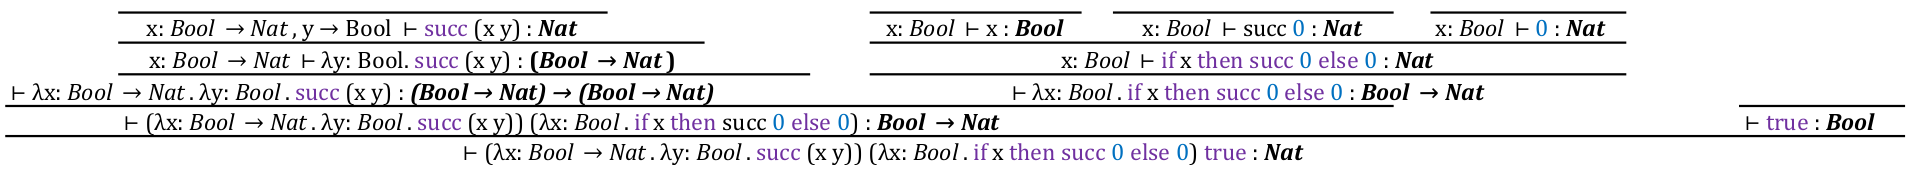
\includegraphics[scale=0.35]{task-1.png}

\vspace{0.5cm}
\hrule
\vspace{0.5cm}


% Выражение 2


\textbf{Выражение 2.} $(\lambda b : Bool. \, \text{\color{purple}if} \, b \, \text{\color{purple}then} (\lambda x : Nat. \, \lambda y : Bool. \, x) \, \text{\color{purple}else} \, (\lambda x : Nat. \, \lambda y: Bool. \, y)) \, {\color{purple} false} \, {\color{blue}0}$

\vspace{0.2cm}

\textit{Дерево вывода типа.}

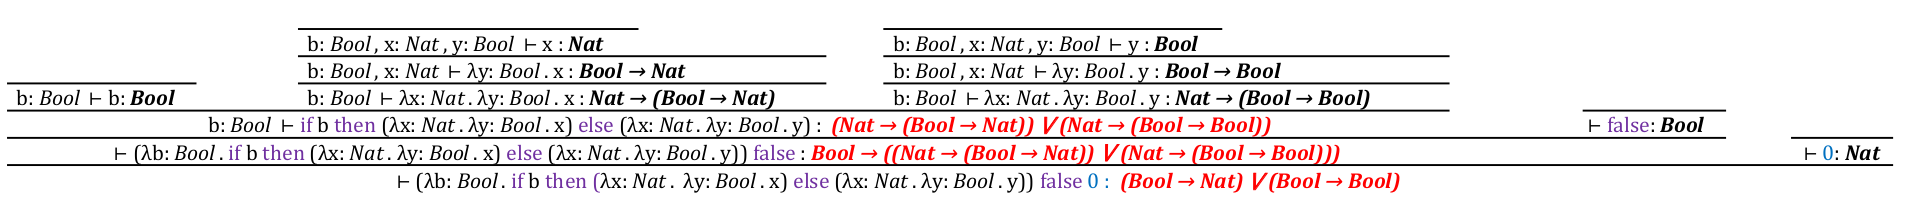
\includegraphics[scale=0.35]{task-2.png}

\vspace{0.5cm}
\hrule
\vspace{0.5cm}

\textit{Ответ.} Данный терм является плохо типизированным.


% Выражение 3


\textbf{Выражение 3.} $(\lambda f : (Nat \rightarrow Nat) \rightarrow (Nat \rightarrow Nat). \, f \, (f \, (\lambda x : Nat. \, x)) \, {\color{blue}0}) (\lambda z : Nat \rightarrow Nat. \, \lambda n : Nat. \, z \, (z \, n))$
\vspace{0.2cm}

\textit{Дерево вывода типа.}

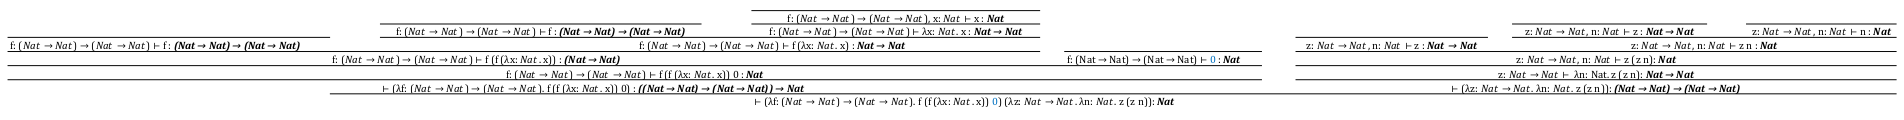
\includegraphics[scale=0.35]{task-3.png}

\vspace{0.5cm}
\hrule
\vspace{0.5cm}


\vfill

\small \textit{Примечание.} Рекомендуется изучить исходный Excel-документ \verb|source.xlsx|.

\end{document}
